\PassOptionsToPackage{unicode=true}{hyperref} % options for packages loaded elsewhere
\PassOptionsToPackage{hyphens}{url}
%
\documentclass[
  ignorenonframetext,
]{beamer}
\usepackage{pgfpages}
\setbeamertemplate{caption}[numbered]
\setbeamertemplate{caption label separator}{: }
\setbeamercolor{caption name}{fg=normal text.fg}
\beamertemplatenavigationsymbolsempty
% Prevent slide breaks in the middle of a paragraph:
\widowpenalties 1 10000
\raggedbottom
\setbeamertemplate{part page}{
  \centering
  \begin{beamercolorbox}[sep=16pt,center]{part title}
    \usebeamerfont{part title}\insertpart\par
  \end{beamercolorbox}
}
\setbeamertemplate{section page}{
  \centering
  \begin{beamercolorbox}[sep=12pt,center]{part title}
    \usebeamerfont{section title}\insertsection\par
  \end{beamercolorbox}
}
\setbeamertemplate{subsection page}{
  \centering
  \begin{beamercolorbox}[sep=8pt,center]{part title}
    \usebeamerfont{subsection title}\insertsubsection\par
  \end{beamercolorbox}
}
\AtBeginPart{
  \frame{\partpage}
}
\AtBeginSection{
  \ifbibliography
  \else
    \frame{\sectionpage}
  \fi
}
\AtBeginSubsection{
  \frame{\subsectionpage}
}
\usepackage{lmodern}
\usepackage{amssymb,amsmath}
\usepackage{ifxetex,ifluatex}
\ifnum 0\ifxetex 1\fi\ifluatex 1\fi=0 % if pdftex
  \usepackage[T1]{fontenc}
  \usepackage[utf8]{inputenc}
  \usepackage{textcomp} % provides euro and other symbols
\else % if luatex or xelatex
  \usepackage{unicode-math}
  \defaultfontfeatures{Scale=MatchLowercase}
  \defaultfontfeatures[\rmfamily]{Ligatures=TeX,Scale=1}
\fi
% use upquote if available, for straight quotes in verbatim environments
\IfFileExists{upquote.sty}{\usepackage{upquote}}{}
\IfFileExists{microtype.sty}{% use microtype if available
  \usepackage[]{microtype}
  \UseMicrotypeSet[protrusion]{basicmath} % disable protrusion for tt fonts
}{}
\makeatletter
\@ifundefined{KOMAClassName}{% if non-KOMA class
  \IfFileExists{parskip.sty}{%
    \usepackage{parskip}
  }{% else
    \setlength{\parindent}{0pt}
    \setlength{\parskip}{6pt plus 2pt minus 1pt}}
}{% if KOMA class
  \KOMAoptions{parskip=half}}
\makeatother
\usepackage{xcolor}
\IfFileExists{xurl.sty}{\usepackage{xurl}}{} % add URL line breaks if available
\IfFileExists{bookmark.sty}{\usepackage{bookmark}}{\usepackage{hyperref}}
\hypersetup{
  pdftitle={Class notes - Bài 2},
  pdfauthor={Kim Văn Thành},
  pdfborder={0 0 0},
  breaklinks=true}
\urlstyle{same}  % don't use monospace font for urls
\newif\ifbibliography
\usepackage{color}
\usepackage{fancyvrb}
\newcommand{\VerbBar}{|}
\newcommand{\VERB}{\Verb[commandchars=\\\{\}]}
\DefineVerbatimEnvironment{Highlighting}{Verbatim}{commandchars=\\\{\}}
% Add ',fontsize=\small' for more characters per line
\newenvironment{Shaded}{}{}
\newcommand{\AlertTok}[1]{\textcolor[rgb]{1.00,0.00,0.00}{\textbf{#1}}}
\newcommand{\AnnotationTok}[1]{\textcolor[rgb]{0.38,0.63,0.69}{\textbf{\textit{#1}}}}
\newcommand{\AttributeTok}[1]{\textcolor[rgb]{0.49,0.56,0.16}{#1}}
\newcommand{\BaseNTok}[1]{\textcolor[rgb]{0.25,0.63,0.44}{#1}}
\newcommand{\BuiltInTok}[1]{#1}
\newcommand{\CharTok}[1]{\textcolor[rgb]{0.25,0.44,0.63}{#1}}
\newcommand{\CommentTok}[1]{\textcolor[rgb]{0.38,0.63,0.69}{\textit{#1}}}
\newcommand{\CommentVarTok}[1]{\textcolor[rgb]{0.38,0.63,0.69}{\textbf{\textit{#1}}}}
\newcommand{\ConstantTok}[1]{\textcolor[rgb]{0.53,0.00,0.00}{#1}}
\newcommand{\ControlFlowTok}[1]{\textcolor[rgb]{0.00,0.44,0.13}{\textbf{#1}}}
\newcommand{\DataTypeTok}[1]{\textcolor[rgb]{0.56,0.13,0.00}{#1}}
\newcommand{\DecValTok}[1]{\textcolor[rgb]{0.25,0.63,0.44}{#1}}
\newcommand{\DocumentationTok}[1]{\textcolor[rgb]{0.73,0.13,0.13}{\textit{#1}}}
\newcommand{\ErrorTok}[1]{\textcolor[rgb]{1.00,0.00,0.00}{\textbf{#1}}}
\newcommand{\ExtensionTok}[1]{#1}
\newcommand{\FloatTok}[1]{\textcolor[rgb]{0.25,0.63,0.44}{#1}}
\newcommand{\FunctionTok}[1]{\textcolor[rgb]{0.02,0.16,0.49}{#1}}
\newcommand{\ImportTok}[1]{#1}
\newcommand{\InformationTok}[1]{\textcolor[rgb]{0.38,0.63,0.69}{\textbf{\textit{#1}}}}
\newcommand{\KeywordTok}[1]{\textcolor[rgb]{0.00,0.44,0.13}{\textbf{#1}}}
\newcommand{\NormalTok}[1]{#1}
\newcommand{\OperatorTok}[1]{\textcolor[rgb]{0.40,0.40,0.40}{#1}}
\newcommand{\OtherTok}[1]{\textcolor[rgb]{0.00,0.44,0.13}{#1}}
\newcommand{\PreprocessorTok}[1]{\textcolor[rgb]{0.74,0.48,0.00}{#1}}
\newcommand{\RegionMarkerTok}[1]{#1}
\newcommand{\SpecialCharTok}[1]{\textcolor[rgb]{0.25,0.44,0.63}{#1}}
\newcommand{\SpecialStringTok}[1]{\textcolor[rgb]{0.73,0.40,0.53}{#1}}
\newcommand{\StringTok}[1]{\textcolor[rgb]{0.25,0.44,0.63}{#1}}
\newcommand{\VariableTok}[1]{\textcolor[rgb]{0.10,0.09,0.49}{#1}}
\newcommand{\VerbatimStringTok}[1]{\textcolor[rgb]{0.25,0.44,0.63}{#1}}
\newcommand{\WarningTok}[1]{\textcolor[rgb]{0.38,0.63,0.69}{\textbf{\textit{#1}}}}
\usepackage{graphicx,grffile}
\makeatletter
\def\maxwidth{\ifdim\Gin@nat@width>\linewidth\linewidth\else\Gin@nat@width\fi}
\def\maxheight{\ifdim\Gin@nat@height>\textheight\textheight\else\Gin@nat@height\fi}
\makeatother
% Scale images if necessary, so that they will not overflow the page
% margins by default, and it is still possible to overwrite the defaults
% using explicit options in \includegraphics[width, height, ...]{}
\setkeys{Gin}{width=\maxwidth,height=\maxheight,keepaspectratio}
\setlength{\emergencystretch}{3em}  % prevent overfull lines
\providecommand{\tightlist}{%
  \setlength{\itemsep}{0pt}\setlength{\parskip}{0pt}}
\setcounter{secnumdepth}{-2}

% set default figure placement to htbp
\makeatletter
\def\fps@figure{htbp}
\makeatother


\title{Class notes - Bài 2}
\author{Kim Văn Thành}
\date{19/08/2020}

\begin{document}
\frame{\titlepage}

\begin{frame}{Lists}
\protect\hypertarget{lists}{}

\begin{itemize}[<+->]
\item
  List là một dạng đặc biệt của Vector.
\item
  Nó chứa các giá trị thuộc các nhóm dữ liệu khác nhau.
\item
  List là dạng trình bày của các R Object đặc biệt. Ví dụ như mô hình
  Linear, mô hình Logistics.
\item
  Những R Object đặc biệt này phải ở dạng list vì nó chứa nhiều thông
  tin khác nhau. Đây cũng là đặc tính nổi trội của list.
\item
  Đặc tính nổi trội của List là chứa đựng rất nhiều thông tin đa dạng
\item
  Việc phân tích dữ liệu sẽ nhanh hơn rất nhiều khi sử dụng các hàm nhóm
  apply() làm việc với R Object dạng list.
\end{itemize}

\end{frame}

\begin{frame}[fragile]{Lists}
\protect\hypertarget{lists-1}{}

\begin{Shaded}
\begin{Highlighting}[]
\NormalTok{x <-}\StringTok{ }\KeywordTok{list}\NormalTok{(}\DecValTok{1}\NormalTok{, }\StringTok{"a"}\NormalTok{, }\OtherTok{TRUE}\NormalTok{, }\DecValTok{1} \OperatorTok{+}\StringTok{ }\NormalTok{4i)}
\NormalTok{x}
\end{Highlighting}
\end{Shaded}

\begin{verbatim}
## [[1]]
## [1] 1
## 
## [[2]]
## [1] "a"
## 
## [[3]]
## [1] TRUE
## 
## [[4]]
## [1] 1+4i
\end{verbatim}

\begin{Shaded}
\begin{Highlighting}[]
\KeywordTok{class}\NormalTok{(x)}
\end{Highlighting}
\end{Shaded}

\begin{verbatim}
## [1] "list"
\end{verbatim}

\end{frame}

\begin{frame}[fragile]{Lists}
\protect\hypertarget{lists-2}{}

Ta có thể tạo List trống với độ dài định sẵn với hàm vector()

\begin{Shaded}
\begin{Highlighting}[]
\NormalTok{x <-}\StringTok{ }\KeywordTok{vector}\NormalTok{(}\DataTypeTok{mode =} \StringTok{"list"}\NormalTok{, }\DataTypeTok{length =} \DecValTok{5}\NormalTok{) }\CommentTok{## bản chất của list chính là vector}
\KeywordTok{print}\NormalTok{(x)}
\end{Highlighting}
\end{Shaded}

\begin{verbatim}
## [[1]]
## NULL
## 
## [[2]]
## NULL
## 
## [[3]]
## NULL
## 
## [[4]]
## NULL
## 
## [[5]]
## NULL
\end{verbatim}

\end{frame}

\begin{frame}[fragile]{Lists}
\protect\hypertarget{lists-3}{}

Khi dùng lệnh View() để xem các Object dạng list ở cửa sổ Source, ta
thấy cách trình bày giá trị của list khác với vector hay matrix

\texttt{x\ \textless{}-\ list(1,\ "a",\ TRUE,\ 1\ +\ 4i)}

\texttt{View(x,\ title\ =\ "List")}

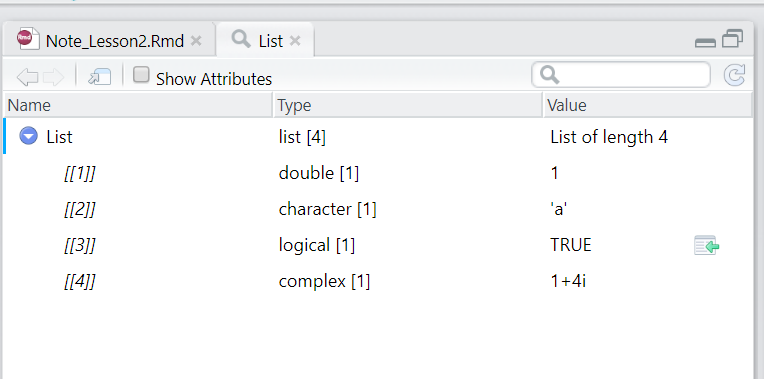
\includegraphics{D:/OneDrive - pnt.edu.vn/Data_Science_in_R/SharingKnowledge/List_in_Source.png}

\end{frame}

\begin{frame}{List}
\protect\hypertarget{list}{}

Số thứ tự giá trị của List được đặt trong dấu ngoặc vuông kép
\emph{{[}{[}số thứ tự{]}{]}}

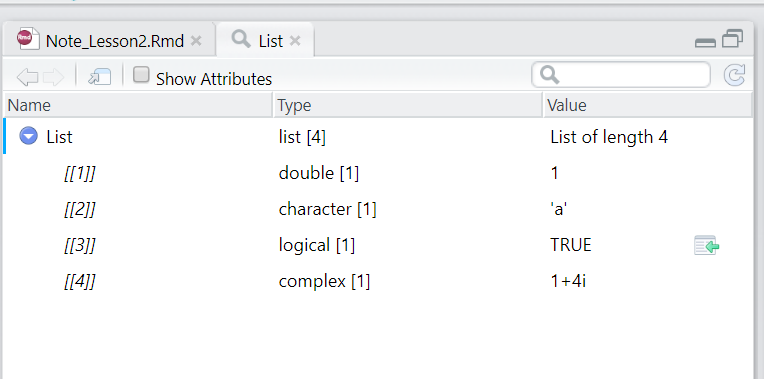
\includegraphics{D:/OneDrive - pnt.edu.vn/Data_Science_in_R/SharingKnowledge/List_in_Source.png}

\end{frame}

\begin{frame}[fragile]{List - Linear model}
\protect\hypertarget{list---linear-model}{}

\begin{Shaded}
\begin{Highlighting}[]
\NormalTok{x <-}\StringTok{ }\KeywordTok{rnorm}\NormalTok{(}\DecValTok{1000}\NormalTok{) ; y <-}\StringTok{ }\KeywordTok{rnorm}\NormalTok{(}\DecValTok{1000}\NormalTok{,}\DecValTok{10}\NormalTok{,}\DecValTok{20}\NormalTok{)}
\NormalTok{model <-}\StringTok{ }\KeywordTok{lm}\NormalTok{(y}\OperatorTok{~}\NormalTok{x)}
\KeywordTok{summary}\NormalTok{(model)}
\end{Highlighting}
\end{Shaded}

\begin{verbatim}
## 
## Call:
## lm(formula = y ~ x)
## 
## Residuals:
##     Min      1Q  Median      3Q     Max 
## -66.662 -12.463   0.325  13.434  62.942 
## 
## Coefficients:
##             Estimate Std. Error t value Pr(>|t|)    
## (Intercept)   9.4325     0.6375  14.797   <2e-16 ***
## x            -0.6272     0.6587  -0.952    0.341    
## ---
## Signif. codes:  0 '***' 0.001 '**' 0.01 '*' 0.05 '.' 0.1 ' ' 1
## 
## Residual standard error: 20.16 on 998 degrees of freedom
## Multiple R-squared:  0.0009078,  Adjusted R-squared:  -9.327e-05 
## F-statistic: 0.9068 on 1 and 998 DF,  p-value: 0.3412
\end{verbatim}

\end{frame}

\begin{frame}[fragile]{List - Linear model}
\protect\hypertarget{list---linear-model-1}{}

\begin{Shaded}
\begin{Highlighting}[]
\NormalTok{model_info <-}\StringTok{ }\KeywordTok{summary}\NormalTok{(model)}
\end{Highlighting}
\end{Shaded}

View(model\_info)

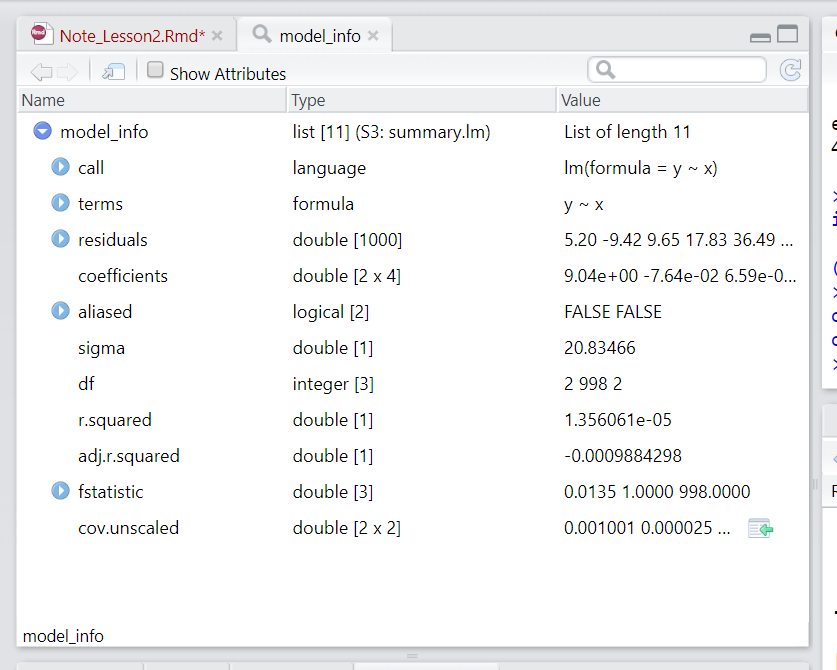
\includegraphics{D:/OneDrive - pnt.edu.vn/Data_Science_in_R/SharingKnowledge/Model_Info.png}

\end{frame}

\begin{frame}{Factor}
\protect\hypertarget{factor}{}

\begin{itemize}[<+->]
\item
  Cấu trúc Factor giúp trình bày dữ liệu dạng định tính theo thứ tự hoặc
  không theo thứ tự.
\item
  Factor quan trọng trong việc xây dựng mô hình, đặc biệt khi làm việc
  với các hàm mô hình như lm() hay glm().
\item
  Factor hoạt động như việc chúng ta gán nhãn giá trị (lab val) cho biến
  số có 2 giá trị (1 và 0 hoặc 2) trong Stata. Ví dụ như gán `Nam' cho
  giá trị 1, và `Nữ' cho giá trị 0 hoặc 2.
\item
  Factor hoạt động ngược lại với Stata. Chúng ta có một biến số nhóm
  character với 2 giá trị là `Nam' và `Nữ'. `Nam' sẽ được gán với giá
  trị 1, `Nữ' được gán với giá trị 2. Nhìn chung, các giá trị sẽ được
  gán với một con số bắt đầu từ số 1.
\item
  Khác với dữ liệu dạng logic (TRUE/FALSE), các con số được gán này
  không thể dùng để tính toán đại số.
\end{itemize}

\end{frame}

\begin{frame}[fragile]{Factor}
\protect\hypertarget{factor-1}{}

Dữ liệu Factor được tạo bằng hàm factor().

\begin{Shaded}
\begin{Highlighting}[]
\NormalTok{x <-}\StringTok{ }\KeywordTok{factor}\NormalTok{(}\KeywordTok{c}\NormalTok{(}\StringTok{"yes"}\NormalTok{,}\StringTok{"yes"}\NormalTok{,}\StringTok{"no"}\NormalTok{,}\StringTok{"yes"}\NormalTok{,}\StringTok{"no"}\NormalTok{))}
\NormalTok{x}
\end{Highlighting}
\end{Shaded}

\begin{verbatim}
## [1] yes yes no  yes no 
## Levels: no yes
\end{verbatim}

\begin{Shaded}
\begin{Highlighting}[]
\KeywordTok{attributes}\NormalTok{(x)}
\end{Highlighting}
\end{Shaded}

\begin{verbatim}
## $levels
## [1] "no"  "yes"
## 
## $class
## [1] "factor"
\end{verbatim}

\begin{Shaded}
\begin{Highlighting}[]
\KeywordTok{table}\NormalTok{(x)}
\end{Highlighting}
\end{Shaded}

\begin{verbatim}
## x
##  no yes 
##   2   3
\end{verbatim}

\end{frame}

\begin{frame}[fragile]{Factor}
\protect\hypertarget{factor-2}{}

Ở phần kết quả, chúng ta thấy `Levels: no yes'. Điều này có nghĩa `no'
tương ứng với 1, `yes' tương ứng với 2. Nếu không có yêu cầu cụ thể, hàm
factor() tự sắp xếp thứ tự theo vị trí của chữ cái đầu trong bảng chữ
cái.

\begin{Shaded}
\begin{Highlighting}[]
\KeywordTok{unclass}\NormalTok{(x)}
\end{Highlighting}
\end{Shaded}

\begin{verbatim}
## [1] 2 2 1 2 1
## attr(,"levels")
## [1] "no"  "yes"
\end{verbatim}

\end{frame}

\begin{frame}[fragile]{Factor}
\protect\hypertarget{factor-3}{}

\begin{Shaded}
\begin{Highlighting}[]
\NormalTok{x <-}\StringTok{ }\KeywordTok{factor}\NormalTok{(}\KeywordTok{c}\NormalTok{(}\StringTok{"yes"}\NormalTok{,}\StringTok{"yes"}\NormalTok{,}\StringTok{"no"}\NormalTok{,}\StringTok{"yes"}\NormalTok{,}\StringTok{"no"}\NormalTok{), }\DataTypeTok{levels =} \KeywordTok{c}\NormalTok{(}\StringTok{"yes"}\NormalTok{,}\StringTok{"no"}\NormalTok{))}
\NormalTok{x}
\end{Highlighting}
\end{Shaded}

\begin{verbatim}
## [1] yes yes no  yes no 
## Levels: yes no
\end{verbatim}

\begin{Shaded}
\begin{Highlighting}[]
\CommentTok{### Hoặc chúng ta có thể sử dụng hàm levels() để xác định đặc tính của dữ liệu. }
\CommentTok{## Điều này tương tự khi ta sử dụng hàm dim() để định dạng vector.}

\KeywordTok{levels}\NormalTok{(x) <-}\StringTok{ }\KeywordTok{c}\NormalTok{(}\StringTok{"no"}\NormalTok{, }\StringTok{"yes"}\NormalTok{) }
\NormalTok{x}
\end{Highlighting}
\end{Shaded}

\begin{verbatim}
## [1] no  no  yes no  yes
## Levels: no yes
\end{verbatim}

\end{frame}

\begin{frame}{Missing data}
\protect\hypertarget{missing-data}{}

\begin{itemize}[<+->]
\item
  Trong R, dữ liệu khuyết được định danh là NA (Not Applicable) hoặc NaN
  (Not a Number).
\item
  Chúng là những từ dành riêng (reserved word) trong R.
\item
  Từ dành riêng là những từ được R hiểu theo nghĩa đặc biệt. Điều này có
  nghĩa

  \begin{itemize}[<+->]
  \tightlist
  \item
    Chúng có vai trò cụ thể.\\
  \item
    Chuyển thành character nếu chúng ta sử dụng dấu nháy đôi.
  \end{itemize}
\end{itemize}

\end{frame}

\begin{frame}[fragile]{Missing data}
\protect\hypertarget{missing-data-1}{}

\begin{Shaded}
\begin{Highlighting}[]
\CommentTok{# Tất cả những chữ cái trong R đều cần dấu nháy đôi. Nếu không có, R sẽ không hiểu. }
\StringTok{"a"}
\end{Highlighting}
\end{Shaded}

\begin{verbatim}
## [1] "a"
\end{verbatim}

\begin{Shaded}
\begin{Highlighting}[]
\NormalTok{x <-}\StringTok{ "a"}
\NormalTok{x}
\end{Highlighting}
\end{Shaded}

\begin{verbatim}
## [1] "a"
\end{verbatim}

\end{frame}

\begin{frame}[fragile]{Missing data}
\protect\hypertarget{missing-data-2}{}

\begin{Shaded}
\begin{Highlighting}[]
\CommentTok{# Tuy nhiên, nó vẫn hiểu Reserved words}
\OtherTok{NA}\NormalTok{; }\KeywordTok{class}\NormalTok{(}\OtherTok{NA}\NormalTok{)}
\end{Highlighting}
\end{Shaded}

\begin{verbatim}
## [1] NA
\end{verbatim}

\begin{verbatim}
## [1] "logical"
\end{verbatim}

\begin{Shaded}
\begin{Highlighting}[]
\OtherTok{NaN}\NormalTok{; }\KeywordTok{class}\NormalTok{(}\OtherTok{NaN}\NormalTok{)}
\end{Highlighting}
\end{Shaded}

\begin{verbatim}
## [1] NaN
\end{verbatim}

\begin{verbatim}
## [1] "numeric"
\end{verbatim}

\begin{Shaded}
\begin{Highlighting}[]
\NormalTok{x <-}\StringTok{ }\OtherTok{Inf}\NormalTok{ ; x ; }\KeywordTok{class}\NormalTok{(x)}
\end{Highlighting}
\end{Shaded}

\begin{verbatim}
## [1] Inf
\end{verbatim}

\begin{verbatim}
## [1] "numeric"
\end{verbatim}

\end{frame}

\begin{frame}{Missing data}
\protect\hypertarget{missing-data-3}{}

\begin{itemize}[<+->]
\tightlist
\item
  Những từ dành riêng thường sử dụng như

  \begin{itemize}[<+->]
  \tightlist
  \item
    Nhóm logical, numeric: TRUE, FALSE\\
  \item
    Nhóm numeric: NaN, Inf, -Inf\\
  \item
    Nhóm tự do (có thể ở tất cả nhóm): NA. Như vậy ta sẽ có numeric NA,
    integer NA, character NA, etc.
  \end{itemize}
\item
  Để kiểm tra một đối tượng có chứa dữ liệu khuyết, ta dùng

  \begin{itemize}[<+->]
  \tightlist
  \item
    Hàm is.na() cho NA\\
  \item
    Hàm is.nan() cho NaN
  \end{itemize}
\end{itemize}

\end{frame}

\begin{frame}[fragile]{Missing data}
\protect\hypertarget{missing-data-4}{}

\begin{Shaded}
\begin{Highlighting}[]
\CommentTok{# Tạo một vector chứa NA}
\NormalTok{x <-}\StringTok{ }\KeywordTok{c}\NormalTok{(}\DecValTok{1}\NormalTok{,}\DecValTok{2}\NormalTok{,}\OtherTok{NA}\NormalTok{,}\DecValTok{10}\NormalTok{,}\DecValTok{3}\NormalTok{)}
\CommentTok{# Trả về một vector logic chỉ ra thành phần nào là NA}
\KeywordTok{is.na}\NormalTok{(x)}
\end{Highlighting}
\end{Shaded}

\begin{verbatim}
## [1] FALSE FALSE  TRUE FALSE FALSE
\end{verbatim}

\begin{Shaded}
\begin{Highlighting}[]
\CommentTok{# Trả về một vector logic chỉ ra thành phần nào là NaN}
\KeywordTok{is.nan}\NormalTok{(x)}
\end{Highlighting}
\end{Shaded}

\begin{verbatim}
## [1] FALSE FALSE FALSE FALSE FALSE
\end{verbatim}

\begin{Shaded}
\begin{Highlighting}[]
\CommentTok{# Bây giờ tạo một vector có cả giá trị NA và NaN}
\NormalTok{x <-}\StringTok{ }\KeywordTok{c}\NormalTok{(}\DecValTok{1}\NormalTok{,}\DecValTok{2}\NormalTok{,}\OtherTok{NaN}\NormalTok{,}\OtherTok{NA}\NormalTok{,}\DecValTok{4}\NormalTok{) ; }\KeywordTok{is.na}\NormalTok{(x) ; }\KeywordTok{is.nan}\NormalTok{(x)}
\end{Highlighting}
\end{Shaded}

\begin{verbatim}
## [1] FALSE FALSE  TRUE  TRUE FALSE
\end{verbatim}

\begin{verbatim}
## [1] FALSE FALSE  TRUE FALSE FALSE
\end{verbatim}

\end{frame}

\begin{frame}{Data frames}
\protect\hypertarget{data-frames}{}

\begin{itemize}[<+->]
\item
  Data frames lưu trữ dữ liệu bảng - một dạng dữ liệu quan trong R.
\item
  Data Frames là một dạng trình bày đặc biệt của list - khi các thành
  phần của list có cùng độ dài.
\item
  Các thành phần của list được xem như là một cột. Độ dài của mỗi thành
  phần trong list là số hàng.
\item
  Khác với matrix, data frames có khá năng lưu trữ các nhóm đối tượng
  khác nhau ở các cột. Trong khi đó, các thành phần trong matrix phải
  cùng nhóm.
\item
  Thậm chí data frame có thê lưu trữ data frame như là một thành phần.
\end{itemize}

\end{frame}

\begin{frame}[fragile]{Data frame}
\protect\hypertarget{data-frame}{}

Data frame có thể được tạo bằng hàm data.frame().

\begin{Shaded}
\begin{Highlighting}[]
\NormalTok{x <-}\StringTok{ }\KeywordTok{data.frame}\NormalTok{(}\DataTypeTok{foo =} \DecValTok{1}\OperatorTok{:}\DecValTok{4}\NormalTok{, }\DataTypeTok{bar =} \KeywordTok{c}\NormalTok{(T,T,F,F)); x}
\end{Highlighting}
\end{Shaded}

\begin{verbatim}
##   foo   bar
## 1   1  TRUE
## 2   2  TRUE
## 3   3 FALSE
## 4   4 FALSE
\end{verbatim}

\begin{Shaded}
\begin{Highlighting}[]
\KeywordTok{dim}\NormalTok{(x) }\CommentTok{# Tương tự như matrix, data frame có dimension}
\end{Highlighting}
\end{Shaded}

\begin{verbatim}
## [1] 4 2
\end{verbatim}

\begin{Shaded}
\begin{Highlighting}[]
\KeywordTok{nrow}\NormalTok{(x) ; }\KeywordTok{ncol}\NormalTok{(x)  }\CommentTok{# number of row, number of collumn}
\end{Highlighting}
\end{Shaded}

\begin{verbatim}
## [1] 4
\end{verbatim}

\begin{verbatim}
## [1] 2
\end{verbatim}

\end{frame}

\begin{frame}{Names}
\protect\hypertarget{names}{}

\begin{itemize}[<+->]
\item
  R Object có thể được đặt tên.
\item
  Việc này sẽ thuận lợi trong việc truy xuất thông tin.
\end{itemize}

\end{frame}

\begin{frame}[fragile]{Names}
\protect\hypertarget{names-1}{}

\begin{Shaded}
\begin{Highlighting}[]
\NormalTok{v <-}\StringTok{ }\DecValTok{1}\OperatorTok{:}\DecValTok{3}
\NormalTok{v }\CommentTok{# Vector nhóm numeric, có ba giá trị 1,2,3}
\end{Highlighting}
\end{Shaded}

\begin{verbatim}
## [1] 1 2 3
\end{verbatim}

\begin{Shaded}
\begin{Highlighting}[]
\KeywordTok{names}\NormalTok{(v)}
\end{Highlighting}
\end{Shaded}

\begin{verbatim}
## NULL
\end{verbatim}

\end{frame}

\begin{frame}[fragile]{Names}
\protect\hypertarget{names-2}{}

\begin{Shaded}
\begin{Highlighting}[]
\CommentTok{# Tương tự như dim() và level(), names() thuộc attributes của R object, và là một vector.}
\KeywordTok{names}\NormalTok{(v) <-}\StringTok{ }\KeywordTok{c}\NormalTok{(}\StringTok{"Ho Chi Minh"}\NormalTok{, }\StringTok{"Ha Noi"}\NormalTok{, }\StringTok{"Da Nang"}\NormalTok{) }
\NormalTok{v }\CommentTok{# Vector nhóm numeric, có ba giá trị 1,2,3 và tên tương ứng là "Hồ Chí Minh", "Hà Nội", "Đà nẵng"}
\end{Highlighting}
\end{Shaded}

\begin{verbatim}
## Ho Chi Minh      Ha Noi     Da Nang 
##           1           2           3
\end{verbatim}

\begin{Shaded}
\begin{Highlighting}[]
\KeywordTok{names}\NormalTok{(v) }\CommentTok{# Vector nhóm character có 3 giá trị}
\end{Highlighting}
\end{Shaded}

\begin{verbatim}
## [1] "Ho Chi Minh" "Ha Noi"      "Da Nang"
\end{verbatim}

\end{frame}

\begin{frame}[fragile]{Names}
\protect\hypertarget{names-3}{}

Matrix cũng có tên hàng và tên cột

\begin{Shaded}
\begin{Highlighting}[]
\NormalTok{m <-}\StringTok{ }\KeywordTok{matrix}\NormalTok{(}\DecValTok{1}\OperatorTok{:}\DecValTok{4}\NormalTok{,}\DataTypeTok{nrow =}\DecValTok{2}\NormalTok{, }\DataTypeTok{ncol =} \DecValTok{2}\NormalTok{) ; m}
\end{Highlighting}
\end{Shaded}

\begin{verbatim}
##      [,1] [,2]
## [1,]    1    3
## [2,]    2    4
\end{verbatim}

\begin{Shaded}
\begin{Highlighting}[]
\KeywordTok{dimnames}\NormalTok{(m)}
\end{Highlighting}
\end{Shaded}

\begin{verbatim}
## NULL
\end{verbatim}

\begin{Shaded}
\begin{Highlighting}[]
\KeywordTok{dimnames}\NormalTok{(m) <-}\StringTok{ }\KeywordTok{list}\NormalTok{(}\KeywordTok{c}\NormalTok{(}\StringTok{"a"}\NormalTok{,}\StringTok{"b"}\NormalTok{),             }\CommentTok{# Tên hàng}
                    \KeywordTok{c}\NormalTok{(}\StringTok{"c"}\NormalTok{,}\StringTok{"d"}\NormalTok{))             }\CommentTok{# Tên cột}
\NormalTok{m}
\end{Highlighting}
\end{Shaded}

\begin{verbatim}
##   c d
## a 1 3
## b 2 4
\end{verbatim}

\end{frame}

\begin{frame}[fragile]{Names}
\protect\hypertarget{names-4}{}

Tên hàng và tên cột có thể được đặt riêng bằng hàm colnames() và
rownames()

\begin{Shaded}
\begin{Highlighting}[]
\KeywordTok{colnames}\NormalTok{(m) <-}\StringTok{ }\KeywordTok{c}\NormalTok{(}\StringTok{'h'}\NormalTok{,}\StringTok{'f'}\NormalTok{)    }\CommentTok{# Tên cột}
\KeywordTok{rownames}\NormalTok{(m) <-}\StringTok{ }\KeywordTok{c}\NormalTok{(}\StringTok{"x"}\NormalTok{,}\StringTok{"z"}\NormalTok{)    }\CommentTok{# Tên hàng}
\NormalTok{m}
\end{Highlighting}
\end{Shaded}

\begin{verbatim}
##   h f
## x 1 3
## z 2 4
\end{verbatim}

\end{frame}

\begin{frame}[fragile]{Names}
\protect\hypertarget{names-5}{}

Ta cũng đặt tên cho từng thành phần trong List

\begin{Shaded}
\begin{Highlighting}[]
\NormalTok{l <-}\StringTok{ }\KeywordTok{list}\NormalTok{(}\DecValTok{1}\NormalTok{,}\DecValTok{2}\NormalTok{,}\DecValTok{3}\NormalTok{); l}
\end{Highlighting}
\end{Shaded}

\begin{verbatim}
## [[1]]
## [1] 1
## 
## [[2]]
## [1] 2
## 
## [[3]]
## [1] 3
\end{verbatim}

\begin{Shaded}
\begin{Highlighting}[]
\KeywordTok{names}\NormalTok{(l)}
\end{Highlighting}
\end{Shaded}

\begin{verbatim}
## NULL
\end{verbatim}

\end{frame}

\begin{frame}[fragile]{Names}
\protect\hypertarget{names-6}{}

\begin{Shaded}
\begin{Highlighting}[]
\NormalTok{l <-}\StringTok{ }\KeywordTok{list}\NormalTok{(}\StringTok{'Ho Chi Minh'}\NormalTok{ =}\StringTok{ }\DecValTok{1}\NormalTok{, }\DataTypeTok{Hanoi =} \DecValTok{2}\NormalTok{, }\DataTypeTok{DaNang =} \DecValTok{3}\NormalTok{); l}
\end{Highlighting}
\end{Shaded}

\begin{verbatim}
## $`Ho Chi Minh`
## [1] 1
## 
## $Hanoi
## [1] 2
## 
## $DaNang
## [1] 3
\end{verbatim}

\begin{Shaded}
\begin{Highlighting}[]
\KeywordTok{names}\NormalTok{(l)}
\end{Highlighting}
\end{Shaded}

\begin{verbatim}
## [1] "Ho Chi Minh" "Hanoi"       "DaNang"
\end{verbatim}

\end{frame}

\begin{frame}[fragile]{Names}
\protect\hypertarget{names-7}{}

Tương tự như vậy cho data frame

\begin{Shaded}
\begin{Highlighting}[]
\NormalTok{df <-}\StringTok{ }\KeywordTok{data.frame}\NormalTok{(}\DecValTok{1}\OperatorTok{:}\DecValTok{5}\NormalTok{,}
                 \KeywordTok{seq}\NormalTok{(}\DecValTok{1}\NormalTok{, }\DecValTok{10}\NormalTok{, }\DataTypeTok{length =} \DecValTok{5}\NormalTok{),}
                 \KeywordTok{c}\NormalTok{(}\StringTok{"a"}\NormalTok{,}\StringTok{"b"}\NormalTok{,}\StringTok{"c"}\NormalTok{,}\StringTok{"d"}\NormalTok{,}\StringTok{"f"}\NormalTok{),}
                 \KeywordTok{sample}\NormalTok{(LETTERS,}\DecValTok{5}\NormalTok{,}\DataTypeTok{replace =} \OtherTok{FALSE}\NormalTok{, }\DataTypeTok{prob =} \OtherTok{NULL}\NormalTok{))}
\KeywordTok{head}\NormalTok{(df,}\DecValTok{2}\NormalTok{)}
\end{Highlighting}
\end{Shaded}

\begin{verbatim}
##   X1.5 seq.1..10..length...5. c..a....b....c....d....f..
## 1    1                   1.00                          a
## 2    2                   3.25                          b
##   sample.LETTERS..5..replace...FALSE..prob...NULL.
## 1                                                V
## 2                                                G
\end{verbatim}

\begin{Shaded}
\begin{Highlighting}[]
\KeywordTok{names}\NormalTok{(df)}
\end{Highlighting}
\end{Shaded}

\begin{verbatim}
## [1] "X1.5"                                            
## [2] "seq.1..10..length...5."                          
## [3] "c..a....b....c....d....f.."                      
## [4] "sample.LETTERS..5..replace...FALSE..prob...NULL."
\end{verbatim}

\end{frame}

\begin{frame}[fragile]{Names}
\protect\hypertarget{names-8}{}

\begin{Shaded}
\begin{Highlighting}[]
\KeywordTok{colnames}\NormalTok{(df) <-}\StringTok{ }\KeywordTok{c}\NormalTok{(}\StringTok{"number_1"}\NormalTok{,}
                  \StringTok{"number_2"}\NormalTok{,}
                  \StringTok{"letter_1"}\NormalTok{,}
                  \StringTok{"letter_2"}\NormalTok{) }\CommentTok{# Tương ứng số cột của df}
\KeywordTok{names}\NormalTok{(df)}
\end{Highlighting}
\end{Shaded}

\begin{verbatim}
## [1] "number_1" "number_2" "letter_1" "letter_2"
\end{verbatim}

\begin{Shaded}
\begin{Highlighting}[]
\KeywordTok{head}\NormalTok{(df,}\DecValTok{2}\NormalTok{)}
\end{Highlighting}
\end{Shaded}

\begin{verbatim}
##   number_1 number_2 letter_1 letter_2
## 1        1     1.00        a        V
## 2        2     3.25        b        G
\end{verbatim}

\end{frame}

\begin{frame}{Tổng kết}
\protect\hypertarget{tux1ed5ng-kux1ebft}{}

\begin{itemize}[<+->]
\item
  Có rất nhiều dạng dữ liệu trong R. Ở phần này chúng ta đã nói về

  \begin{itemize}[<+->]
  \tightlist
  \item
    Nhóm cơ bản: Numeric, logical, character, integer, complex
  \item
    Vector, lists
  \item
    Factor
  \item
    Missing values
  \item
    Data frames và Matrix
  \end{itemize}
\item
  Tất cả R Object đều có attributes để mô tả chúng. Một trong số đó là
  names, dimension đối với data frame và matrix, và level đối với
  factor.
\end{itemize}

\end{frame}

\begin{frame}{Cám ơn mọi người đã chú ý lắng nghe}
\protect\hypertarget{cuxe1m-ux1a1n-mux1ecdi-ngux1b0ux1eddi-ux111uxe3-chuxfa-uxfd-lux1eafng-nghe}{}

\includegraphics{Lesson2_files/figure-beamer/unnamed-chunk-20-1.pdf}

\end{frame}

\end{document}
